\documentclass[12pt,letterpaper]{article}


\newcommand{\studentname}{Ben Bassett}
\newcommand{\labpartner}{Katrina Sumarli}

\title{\textsc{Lab 02: Harmonic Oscillator with Air Drag}}
\newcommand{\shorttitle}{Harmonic Oscillator with Drag}

\newcommand{\course}{PHY310}
\newcommand{\labdate}{09-10-2024}

%------------------------------------------------------------------------------------------------------------

\usepackage[letterpaper,left=1in,right=1in,bottom=1in,top=1in]{geometry}
\usepackage{fancyhdr}
\usepackage{subfigure}
\usepackage{graphicx}
\usepackage{amsmath}
\usepackage{cleveref}
\usepackage{booktabs}
\usepackage[british]{babel}
\usepackage[square,comma,numbers,sort&compress]{natbib}
\usepackage{csvsimple}
\usepackage{graphicx}
\usepackage{pgfplotstable}
\usepackage{textcomp,gensymb}
\usepackage{array}
\usepackage{tabu}
\usepackage{multirow}
\usepackage{url}
\usepackage{lipsum}
\pgfplotsset{compat=1.9}% supress warning
\begin{document}

%------------------------------------------------------------------------------------------------------------

\setlength{\parindent}{1em}
\setlength{\parskip}{0.5em}
\author{\course~Lab Journal \\ \\ \studentname\,\& \labpartner}
\date{\labdate}

\renewcommand\abstractname{Summary}

\pagestyle{fancy}
\fancyhead{}
\fancyhead[l]{\course:~\shorttitle}
\fancyhead[r]{\studentname}
\fancyfoot{}
\fancyfoot[C]{\thepage}
\renewcommand{\headrulewidth}{0pt}
\renewcommand{\footrulewidth}{0pt}

\renewcommand\bibname{References}

%------------------------------------------------------------------------------------------------------------

\renewcommand\abstractname{Abstract}
\maketitle

% COMMENT IN IF ASKED TO SUBMIT REPORT WITH ABSTRACT
%\begin{abstract}
%Maximum 200 words.
%\end{abstract}

\section{Purpose}
This lab aimed to measure the coefficient of air drag as a function of cross-sectional area.

\section{Experimental Apparatus}

We were given a metal spring, cardstock paper, weights, string, scissors, a (drawing) compass, and a retort stand with a horizontal clamp. Our general setup is illustrated in Figure \ref{fig:setup}.

 \begin{figure}[h]
     \centering
     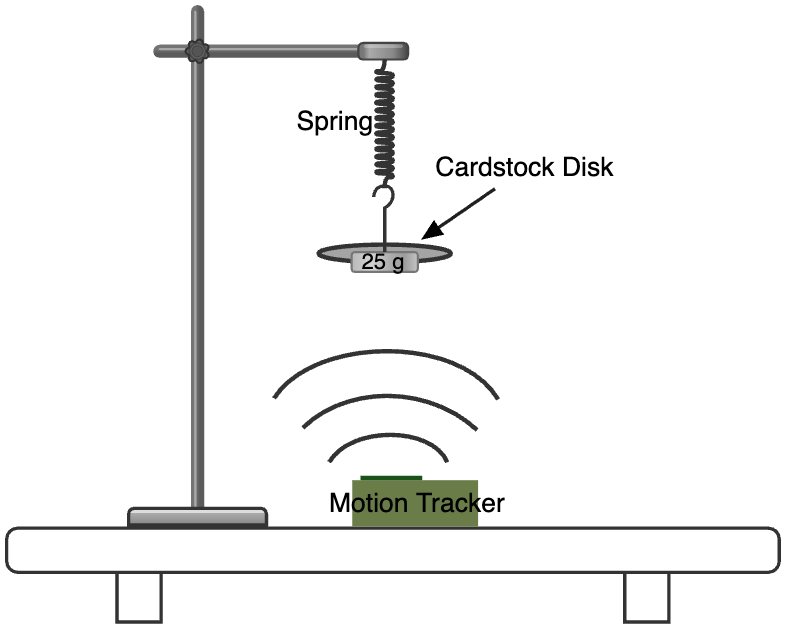
\includegraphics[width=4in]{images/setup.png}
     \caption{A diagram of our experimental setup}
     \label{fig:setup}
 \end{figure}

% \pagebreak
\section{Procedure}

 We used the compass and scissors to cut out four (4) circles of 4cm, 6cm, 8cm, and 10cm. We hung the spring vertically on the horizontal retort clamp, and measured it's equilibrium position. Then we attached the weight hanger (5g) and placed 40g of weight on it. We then measured the new equilibrium position. Then we reduced the total weight on the spring to 25g to capture more exaggerated data, placed the motion sensor beneath, and did 5 30-second motion recordings. The first one had only the 25g, but the second had the 4cm disk, the third the 6cm disk, the fourth the 8cm disk, and the fifth the 10cm disk. On each run, we held the spring as far up as possible, so that the spring was at it's 0g equilibrium position. We then began recording and released it.

\section{Results}

$e^{t-x}$

\begin{equation}
    F_D=3\pi \mu Dv
\end{equation}

\begin{figure}[!htb]
\centering
\begin{subfigure}[b]{0.32\textwidth}
  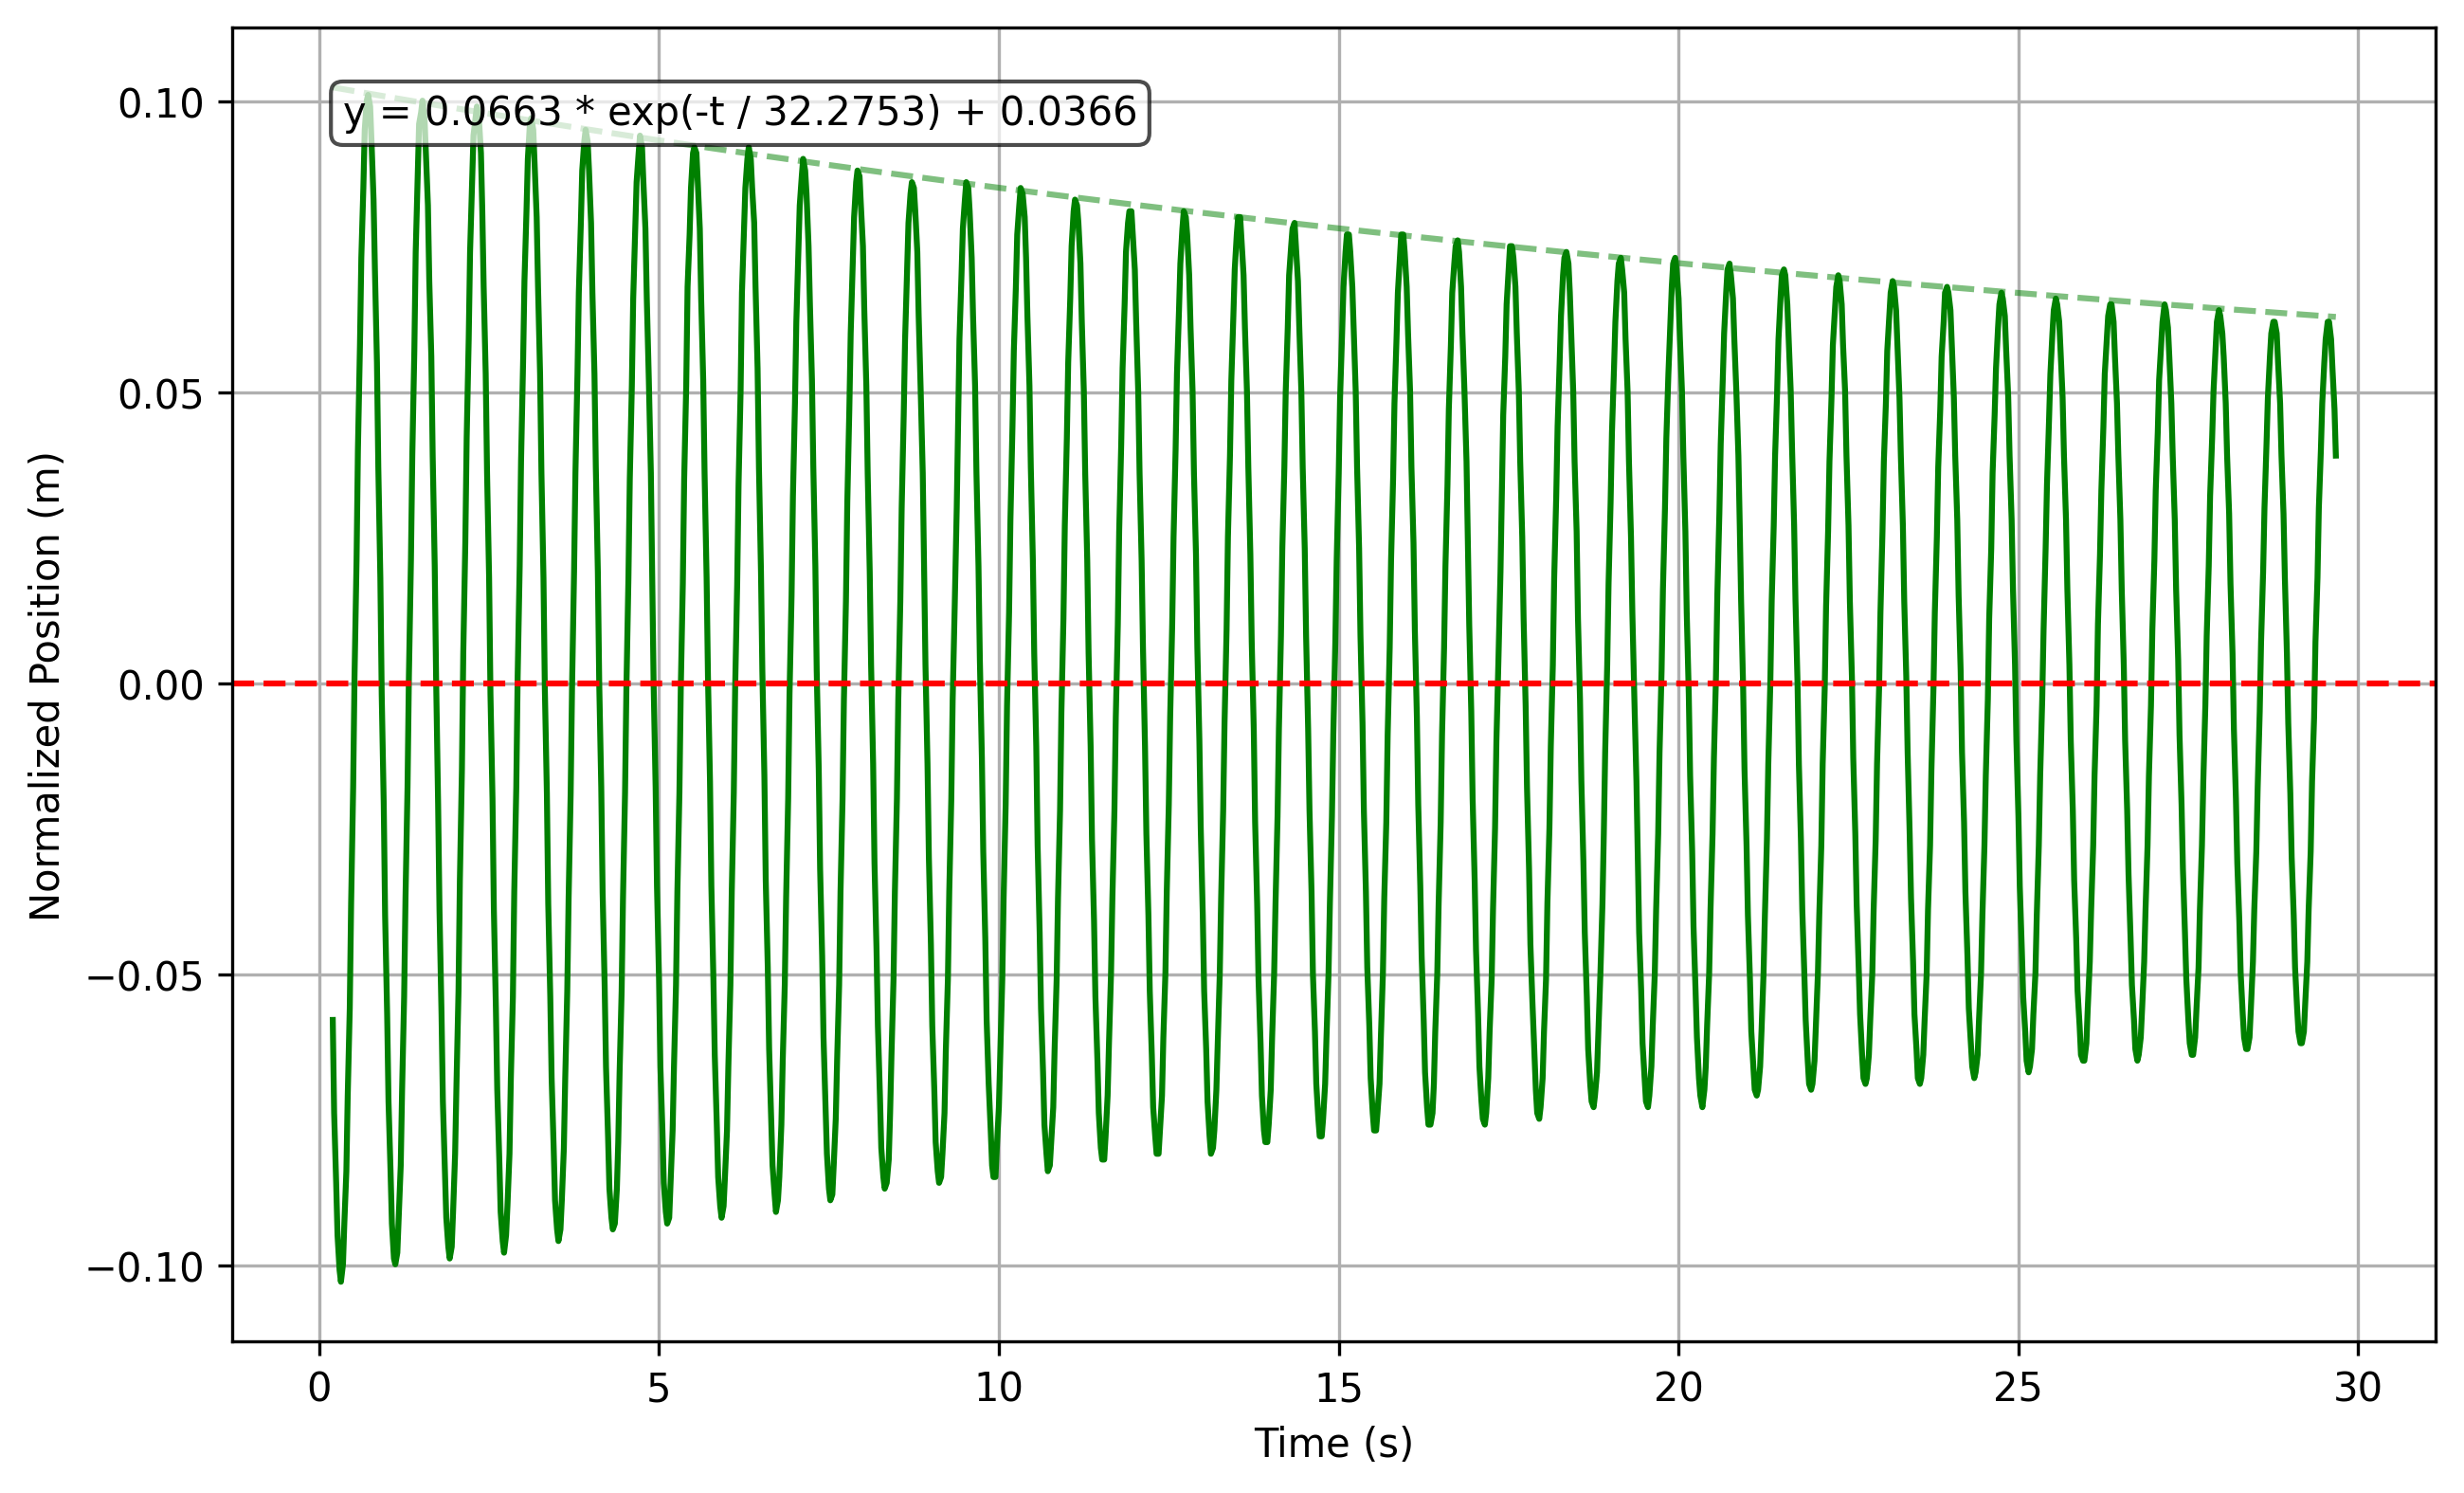
\includegraphics[width=\linewidth]{images/2cm.png}
  \caption{Spring with only 25g}\label{fig:2cm}
\end{subfigure}
\hfill
\begin{subfigure}[b]{0.32\textwidth}
  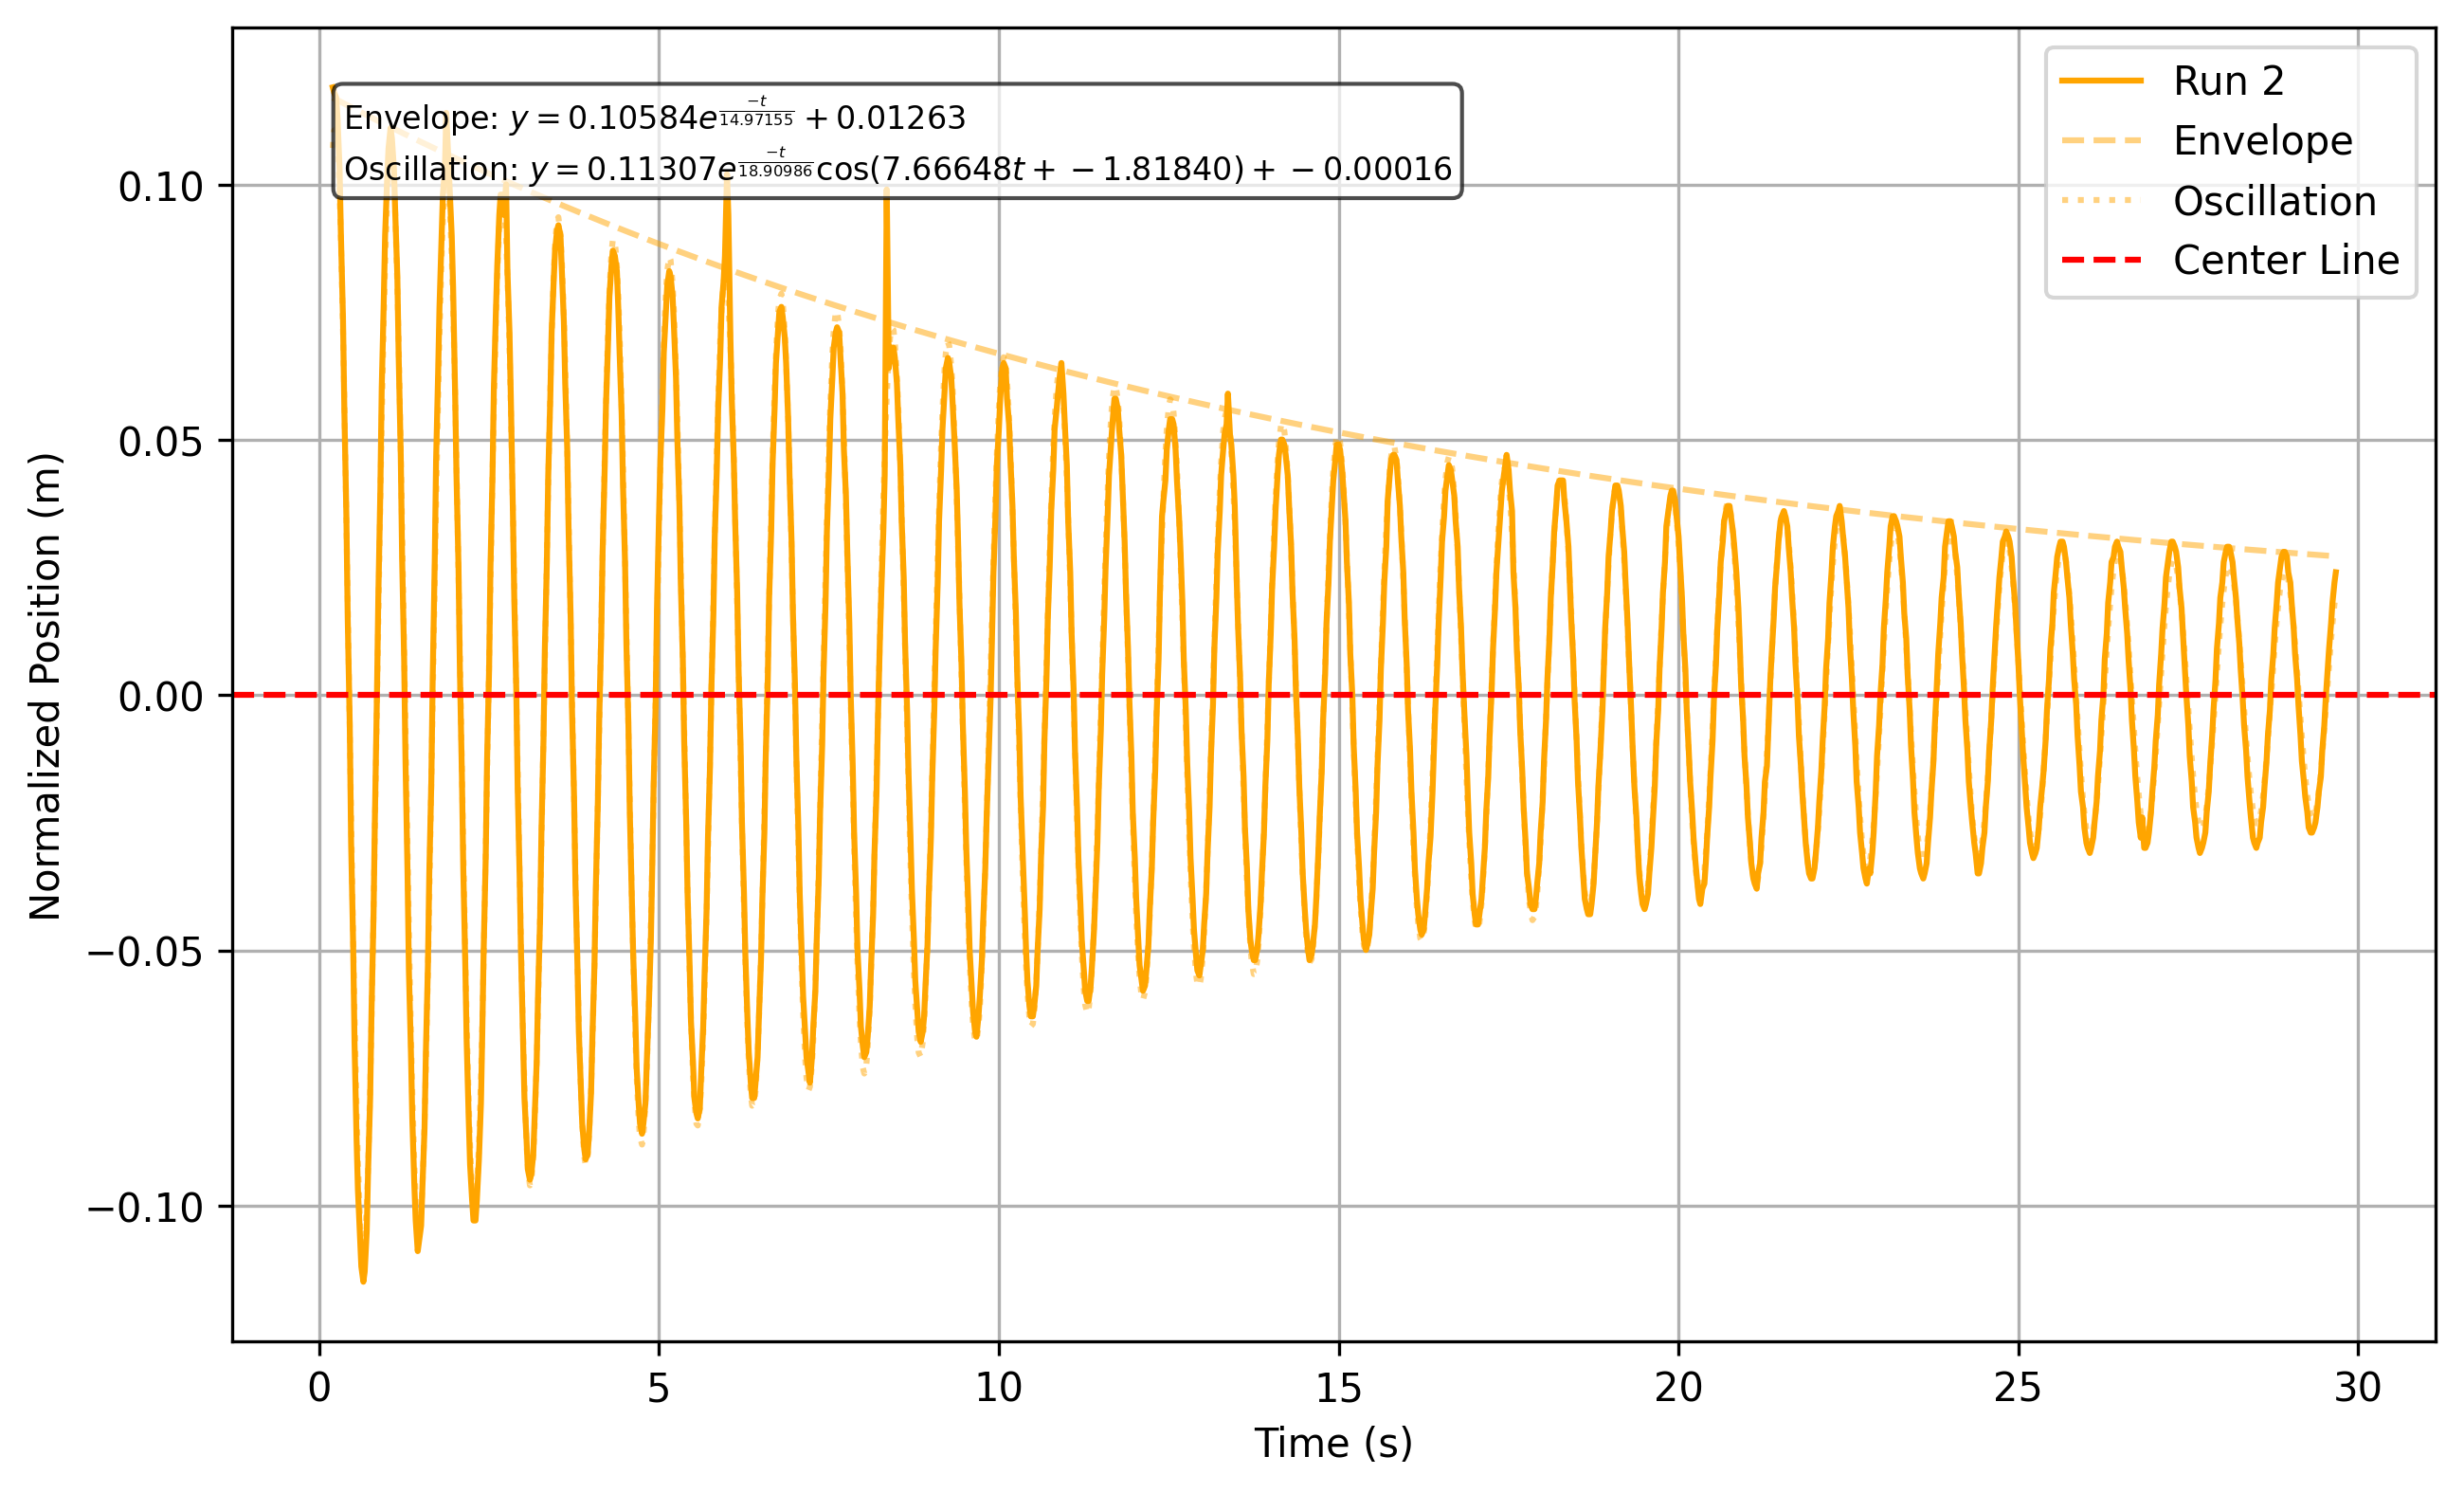
\includegraphics[width=\linewidth]{images/4cm.png}
  \caption{Spring with 25g and a 4cm disk}\label{fig:4cm}
\end{subfigure}
\hfill
\begin{subfigure}[b]{0.32\textwidth}
  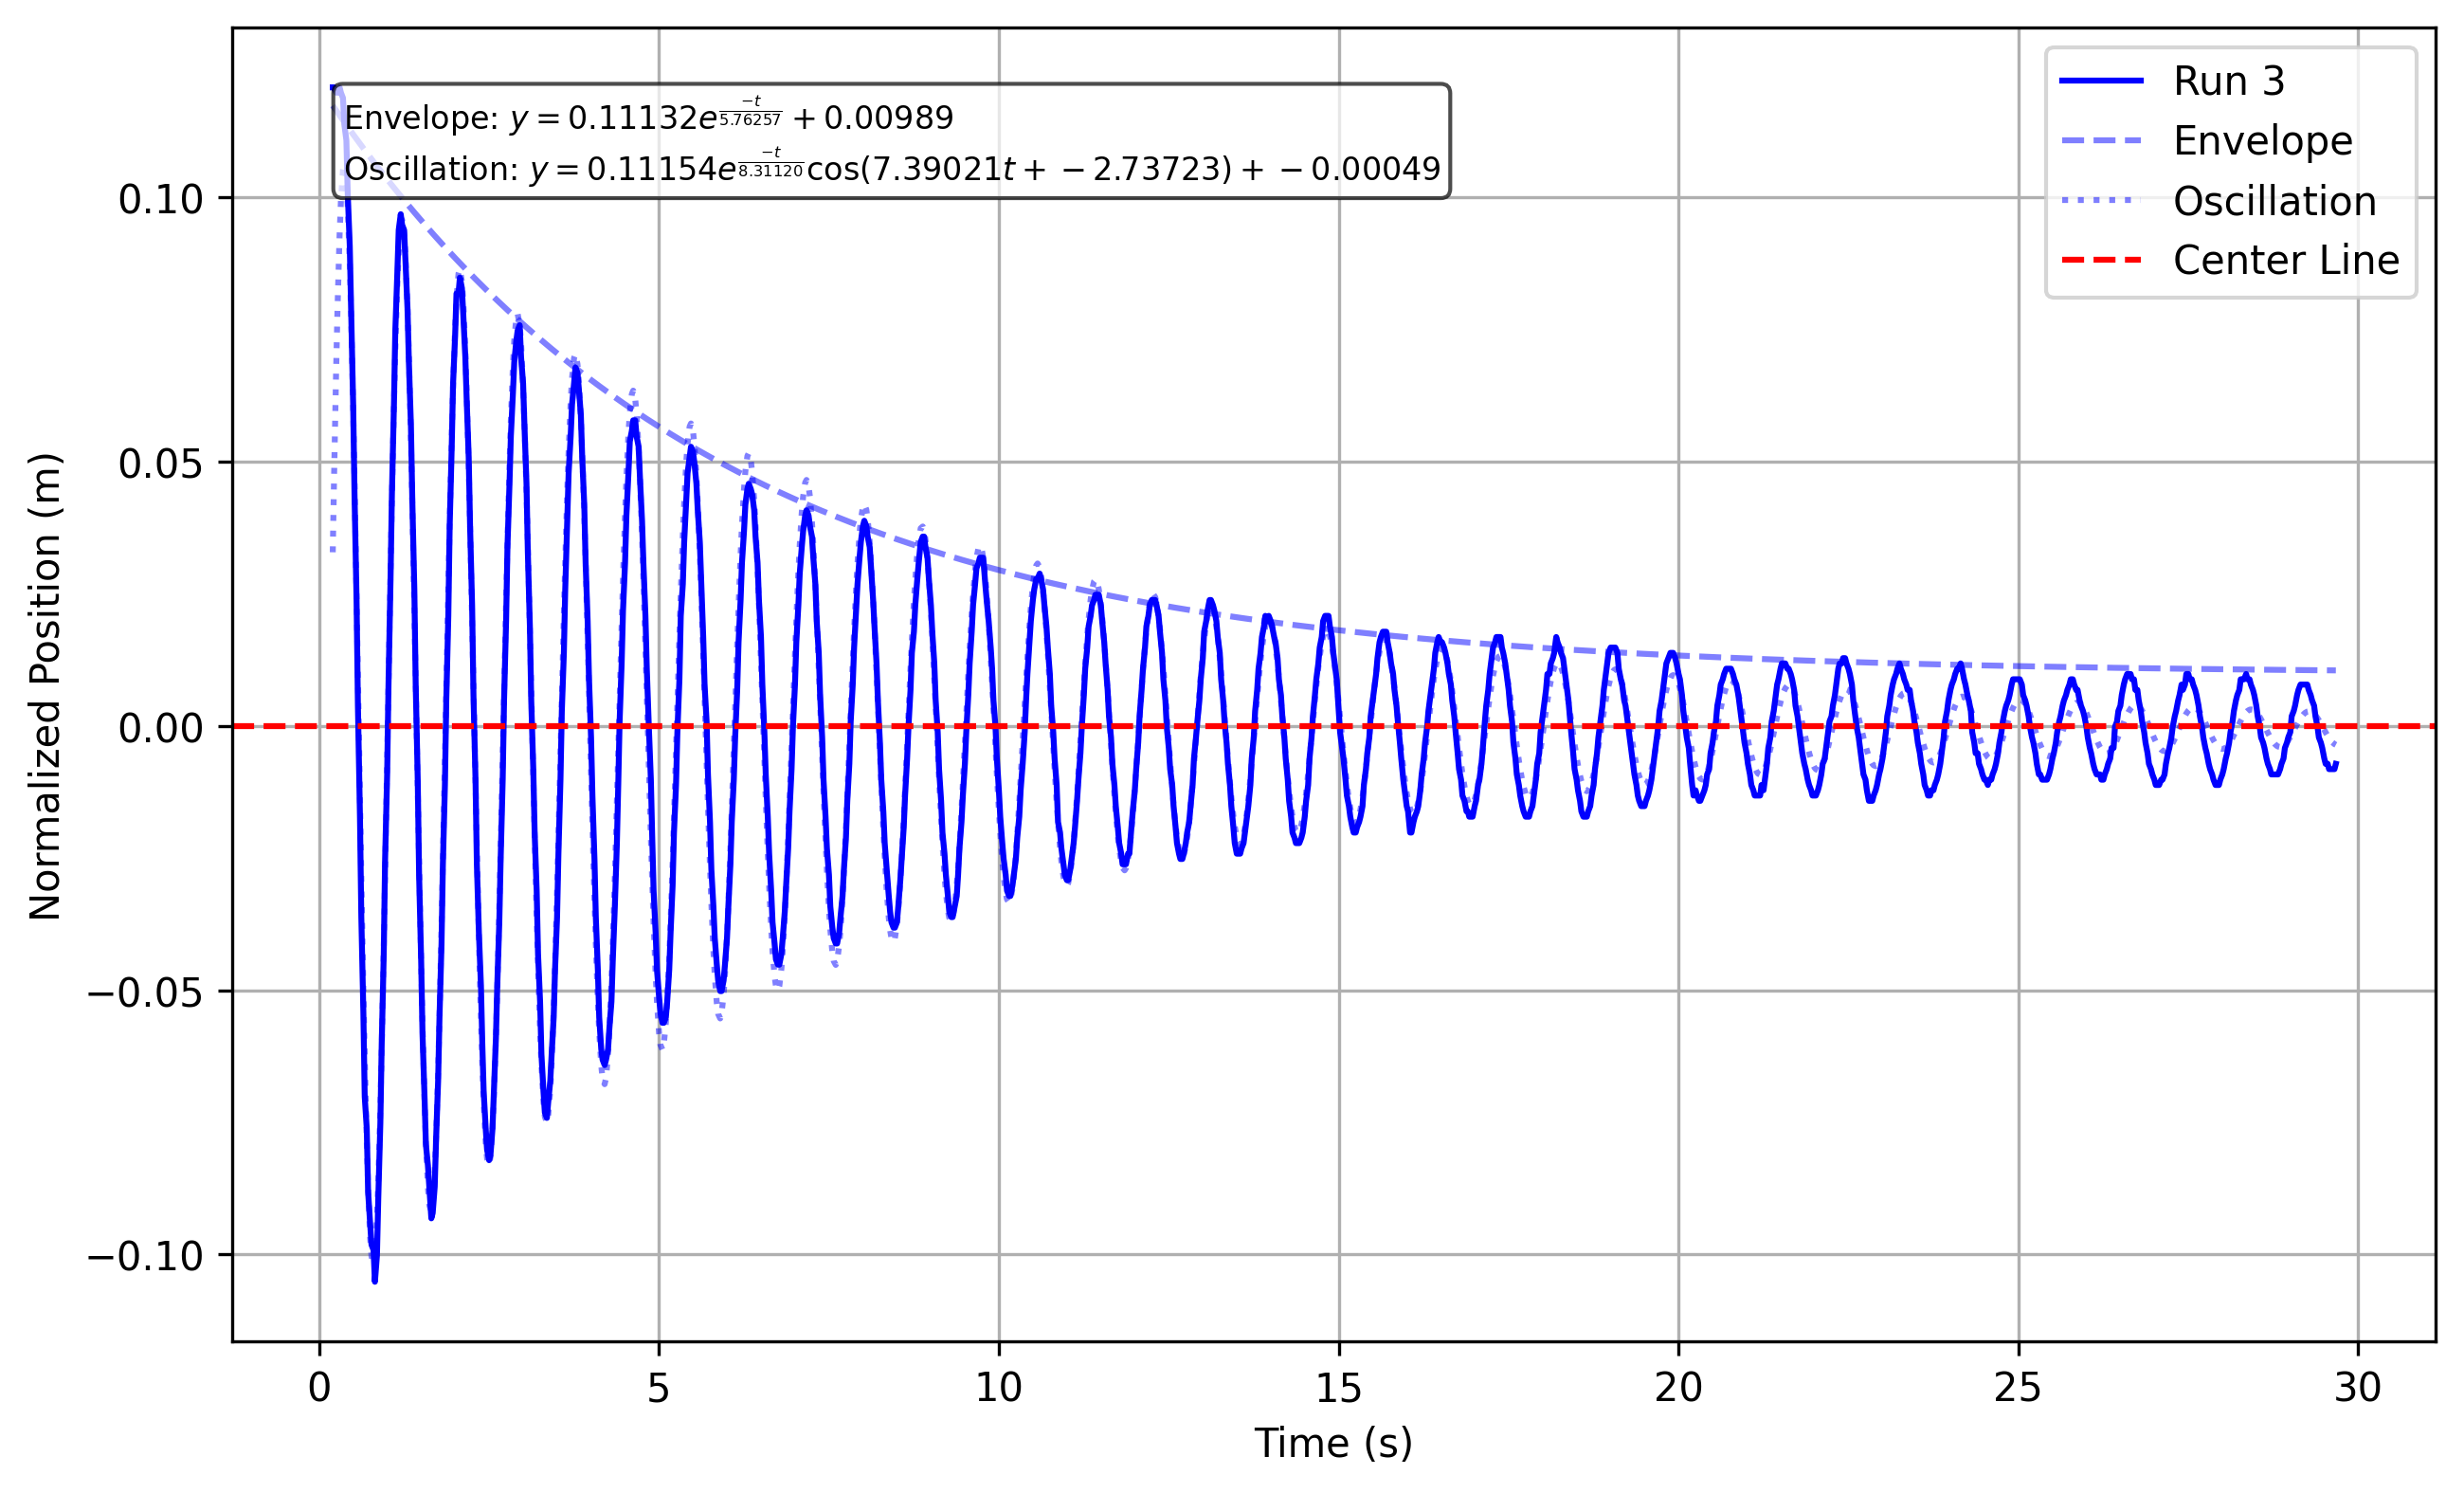
\includegraphics[width=\linewidth]{images/6cm.png}
  \caption{Spring with 25g and a 6cm disk}\label{fig:6cm}
\end{subfigure}

\vspace{0.5cm}

\begin{subfigure}[b]{0.32\textwidth}
  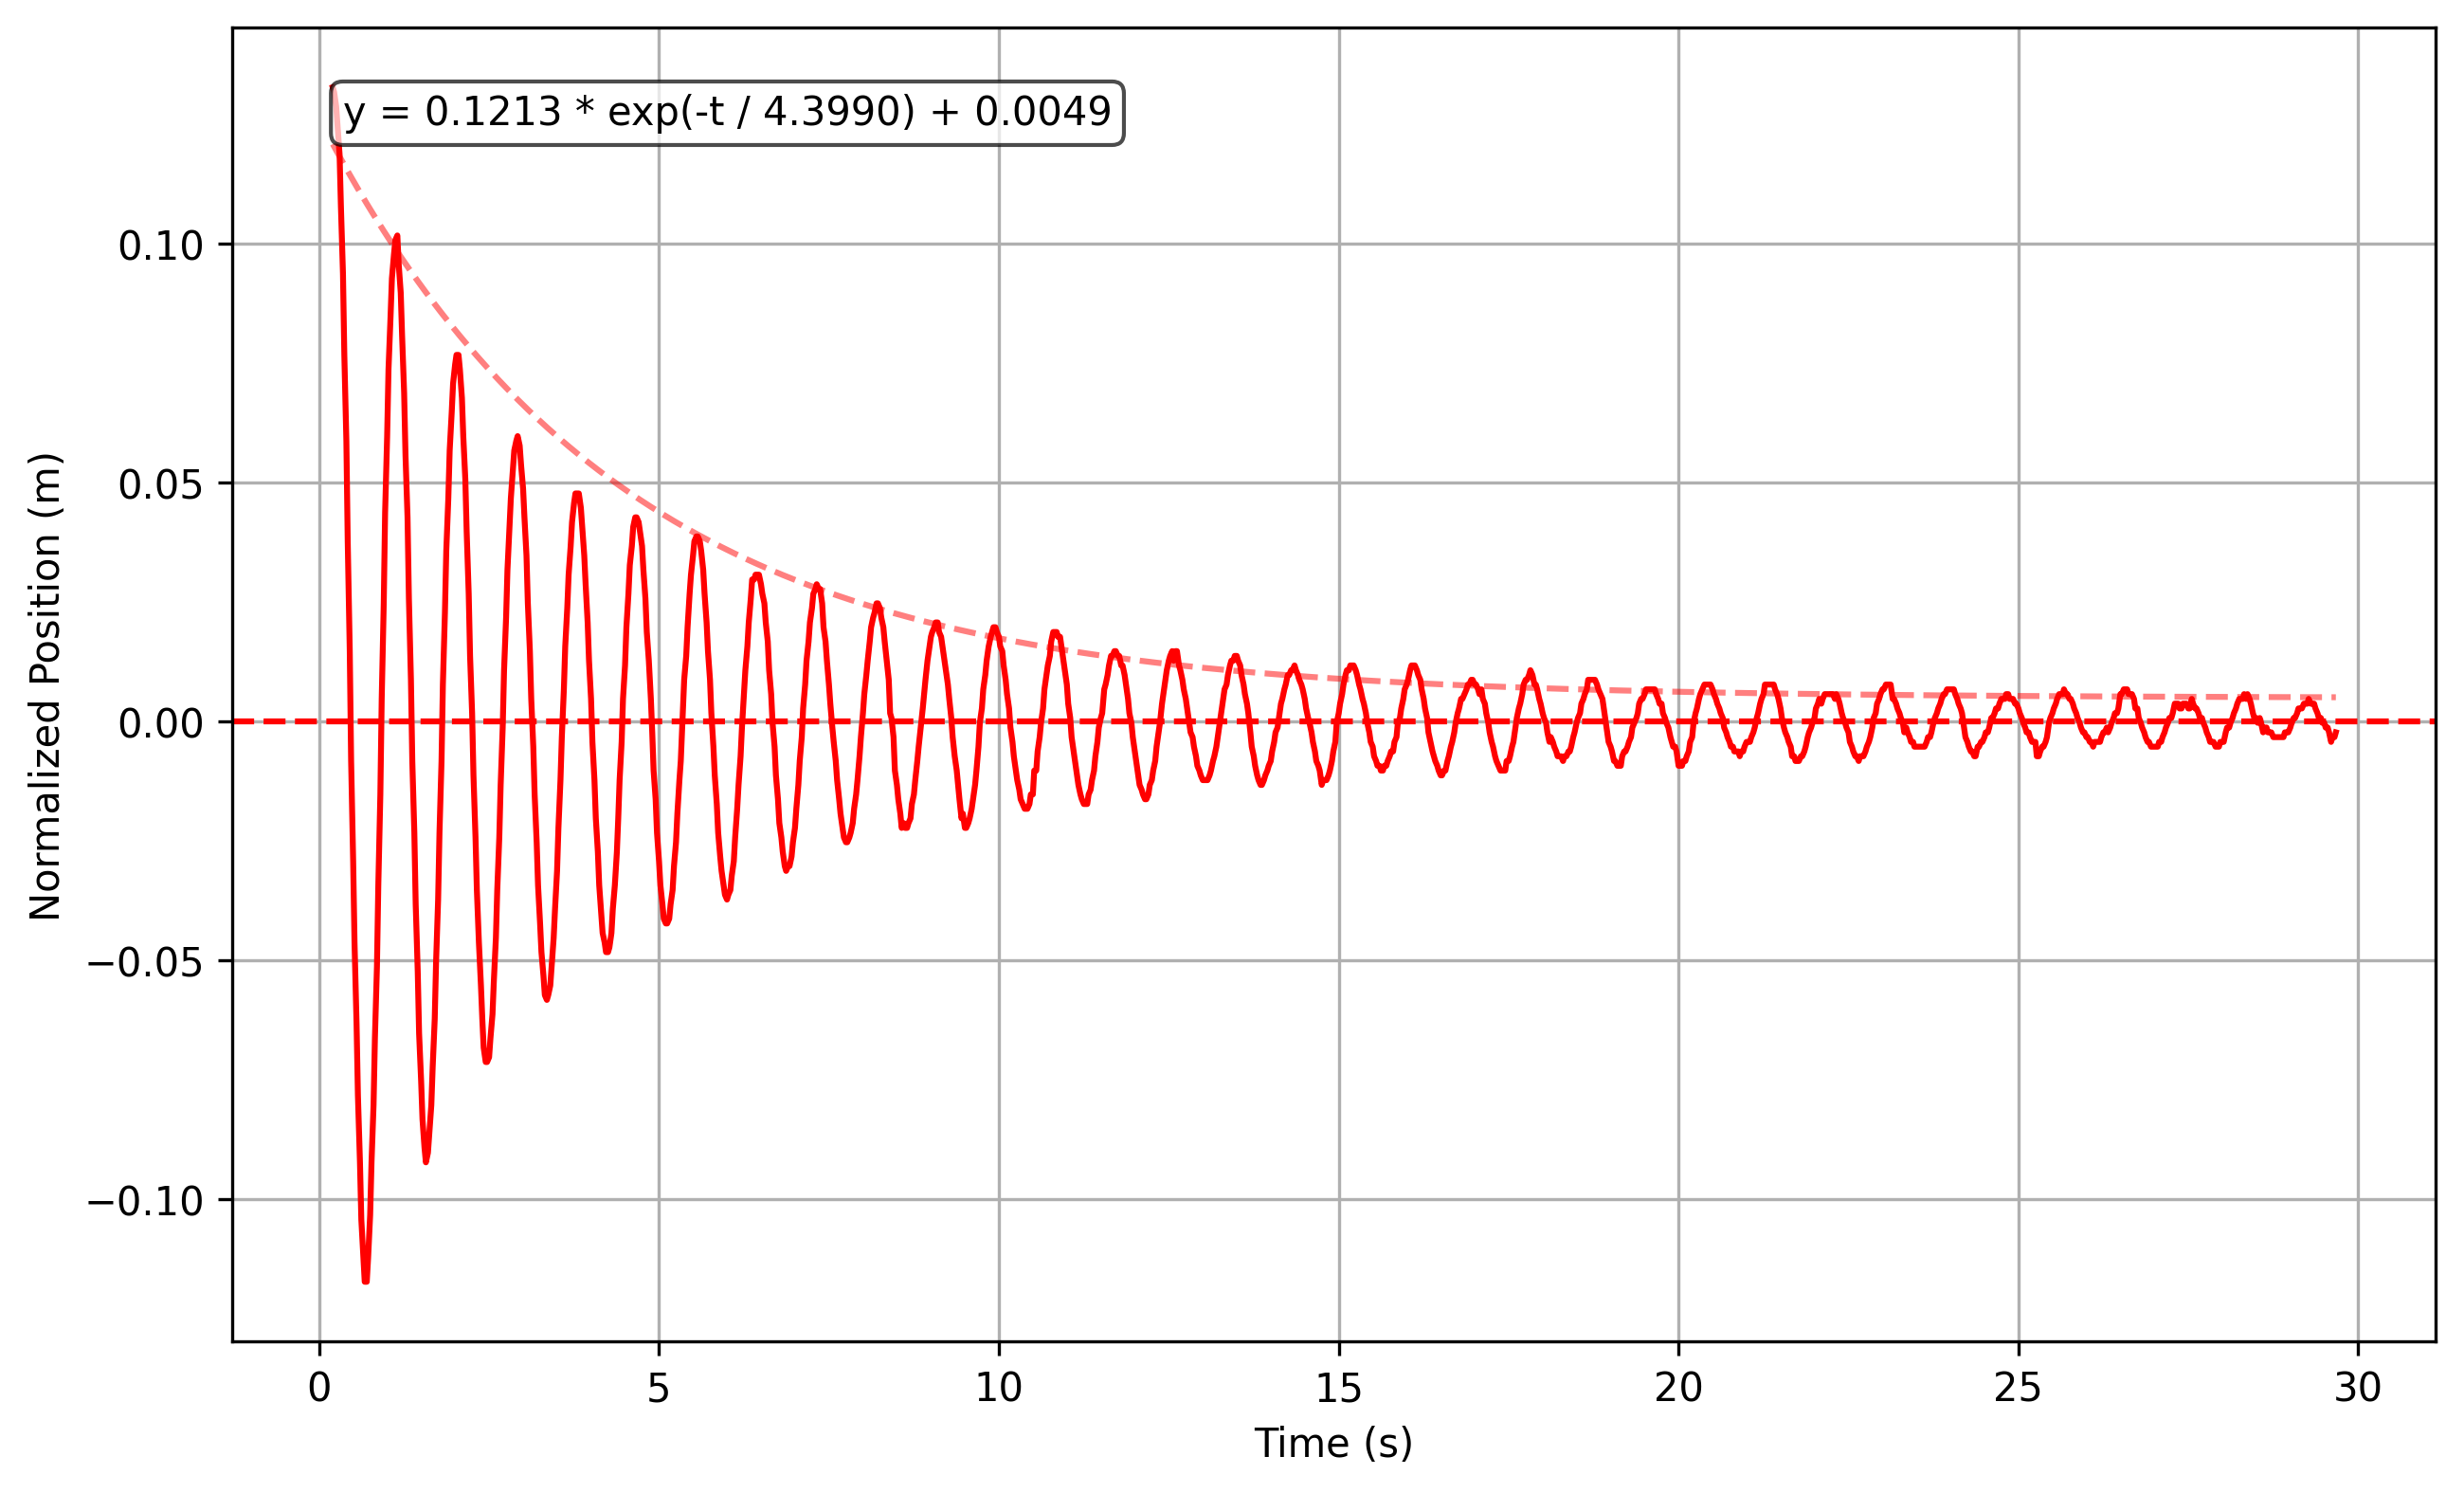
\includegraphics[width=\linewidth]{images/8cm.png}
  \caption{Spring with 25g and an 8cm disk}\label{fig:8cm}
\end{subfigure}
\hfill
\begin{subfigure}[b]{0.32\textwidth}
  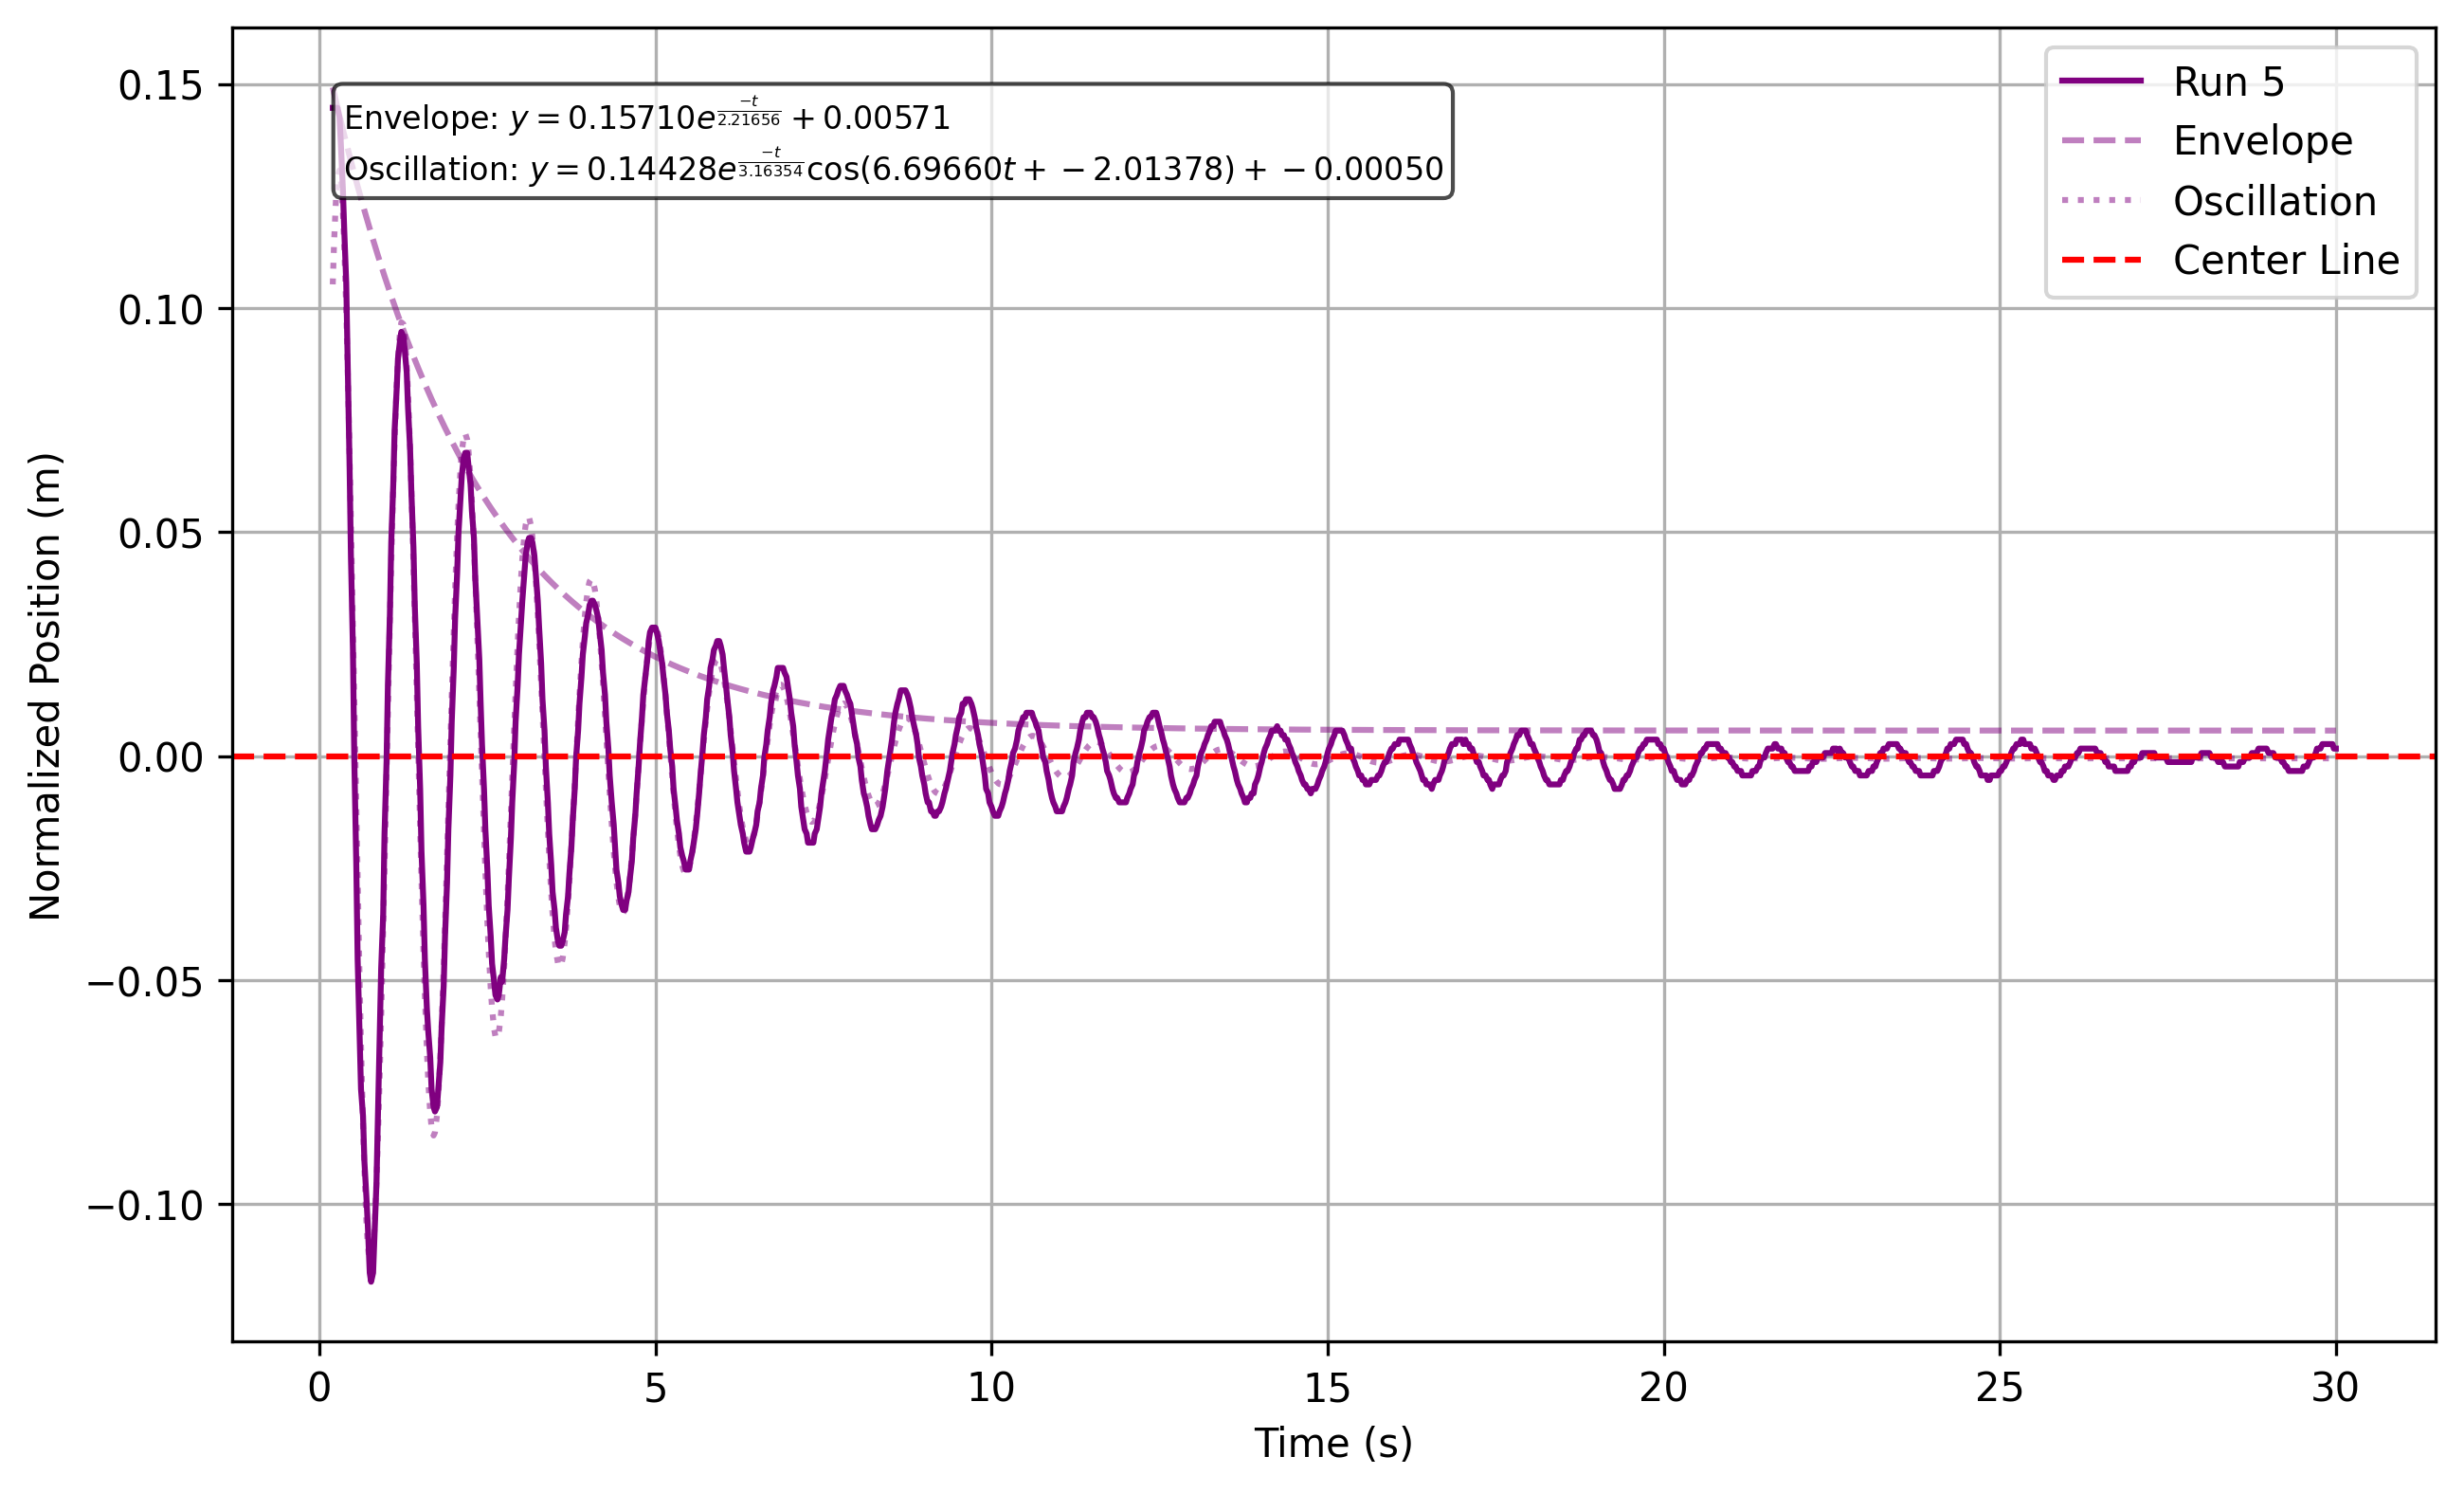
\includegraphics[width=\linewidth]{images/10cm.png}
  \caption{Spring with 25g and a 10cm disk}\label{fig:10cm}
\end{subfigure}
\caption{Spring oscillations with different disk sizes}
\label{fig:all_disks}
\end{figure}

\section{Conclusions}

\lipsum[1]


% \bibliographystyle{unsrtnat}
% \bibliography{references}

\end{document}
